%--------------------------------------------------------------------%
%
% Berkas utama templat LaTeX.
%
% @author Petra Barus, Peb Ruswono Aryan
% updated by Dionesius Agung (2020)
%--------------------------------------------------------------------%
%
% Berkas ini berisi struktur utama dokumen LaTeX yang akan dibuat.
%
%--------------------------------------------------------------------%

\documentclass[12pt, a4paper, onecolumn, oneside, final]{report}

%-------------------------------------------------------------------%
%
% Konfigurasi dokumen LaTeX untuk laporan tesis IF ITB
%
% @author Petra Barus
% updated by Dionesius Agung (2020)
%-------------------------------------------------------------------%
%
% Berkas asli berasal dari Steven Lolong
%
%-------------------------------------------------------------------%

%%%%%%%%%%%%%%%%%%%%%%%%%%%%%%%%%%%%
%  DOCUMENT LAYOUT AND FORMATTING  %
%%%%%%%%%%%%%%%%%%%%%%%%%%%%%%%%%%%%
% Document layout
\usepackage[top=3cm,bottom=3cm,left=4cm,right=3cm,a4paper]{geometry}

% Uncomment these two packages if you want to use
%  the Times New Roman font for your document
% \usepackage{mathptmx}
% \usepackage{newtxtext}

% Judul bahasa Indonesia
\usepackage[bahasa]{babel}

% Spacing 1.5
\usepackage{setspace}
\renewcommand{\baselinestretch}{1.5}

% Prevent overfull (or underfull) if possible
%\setlength{\emergencystretch}{25pt}

% Avoid widow and orphan lines if possible
\widowpenalty=500
\clubpenalty=10000

% Hyphenation penalty
%--------------------------------------------------------------------%
%
% Hyphenation untuk Bahasa Indonesia
%
% @author Petra Barus
%
%--------------------------------------------------------------------%
%
% Secara otomatis LaTeX dapat langsung memenggal kata dalam dokumen,
% tapi sering kali terdapat kesalahan dalam pemenggalan kata. Untuk
% memperbaiki kesalahan pemenggalan kata tertentu, cara pemenggalan
% kata tersebut dapat ditambahkan pada dokumen ini. Pemenggalan
% dilakukan dengan menambahkan karakter '-' pada suku kata yang
% perlu dipisahkan.
%
% Contoh pemenggalan kata 'analisa' dilakukan dengan 'a-na-li-sa'
%
%--------------------------------------------------------------------%

\hyphenation {
	% A
	%
	a-na-li-sa
	a-pli-ka-si

	% B
	%
	be-be-ra-pa
	ber-ge-rak

	% C
	%
	ca-ri

	% D
	%
	da-e-rah
	di-nya-ta-kan
	de-fi-ni-si

	% E
	%
	e-ner-gi
	eks-klu-sif

	% F
	%
	fa-si-li-tas

	% G
	%
	ga-bung-an

	% H
	%
	ha-lang-an

	% I
	% 
	i-nduk

	% J
	%
	ka-me-ra
	kua-li-tas

	% K
	%

	% L
	%

	% M
	%

	% N
	%

	% O
	%

	% P
	%

	% Q
	%

	% R
	%

	% S
	%

	% T
	% 

	% U
	%

	% V
	%

	% W
	%

	% X
	%

	% Y
	% 

	% Z
	%
}

\hyphenpenalty=1000
\tolerance=1
\sloppy


%%%%%%%%%%%%%%%%%%%%%%%%%%%%%%%
%  BIBLIOGRAPHY AND CITATION  %
%%%%%%%%%%%%%%%%%%%%%%%%%%%%%%%
% use package biblatex
\usepackage[backend=bibtex,
	bibstyle=authoryear,
	citestyle=authoryear,
	sorting=nyt,
	url=false,
	maxcitenames=2,
	maxnames=2,
	dashed=false,
	giveninits=true]{biblatex}
\DeclareNameAlias{author}{last-first}

% Translate bibliography strings ke bahasa indonesia
%   (karena 'bahasa' belum di-support)
\DefineBibliographyStrings{english}{%
	bibliography = {Daftar Pustaka},
	references = {Referensi},
	and = {dan},
	techreport = {Dok. teknis},
	phdthesis = {Disertasi doktoral\adddot},
	andothers = {dkk\adddot}
}

% Field berikut tidak ditulis di daftar pustaka
\AtEveryBibitem{\clearfield{issn}}
\AtEveryBibitem{\clearfield{isbn}}
\AtEveryBibitem{\clearfield{month}}
\AtEveryBibitem{\clearfield{doi}}

% Format entri daftar pustaka

%% Beri titik setelah judul
\DeclareFieldFormat
[article,inbook,incollection,inproceedings,
	patent,unpublished,misc]
{title}{#1\isdot}

%% Judul buku ditulis italic
\DeclareFieldFormat
[thesis]
{title}{\emph{#1}\isdot}

%% Hilangkan kata "Dalam:" di antara judul artikel dan judul jurnal
\renewbibmacro{in:}{}

%% Format penulisan volume dan nomor pada jurnal: vol(num) e.g. 5(1)
\renewbibmacro*{volume+number+eid}{%
	\printfield{volume}%
	\printfield{number}%
	\setunit{\addcomma\space}%
	\printfield{eid}}
\DeclareFieldFormat[article]{number}{\mkbibparens{#1}}

% Format citation
\renewcommand*{\nameyeardelim}{\addcomma\space}

% Setting spasi di halaman daftar pustaka
\setlength\bibitemsep{0.5\baselineskip}


%%%%%%%%%%%%%%
%  PACKAGES  %
%%%%%%%%%%%%%%
\usepackage[utf8]{inputenc}
\usepackage{graphicx}
\usepackage{titling}
\usepackage{blindtext}
\usepackage{sectsty}
\usepackage{chngcntr}
\usepackage{etoolbox}
\usepackage{hyperref}       % Package untuk link di daftar isi.
\usepackage{titlesec}       % Package Format judul
\usepackage{parskip}
\usepackage{booktabs}
\usepackage{tabularx}
\usepackage[chapter]{algorithm} % untuk algoritma
\usepackage{algpseudocode} 		  % untuk algoritma


%%%%%%%%%%%%%%$$%%%%%%%%%
%  CHAPTER AND SECTION  %
%%%%%%%%%%%%%%%%$$%%%%%%%
% Format judul bab
\chapterfont{\centering \large}
\titleformat{\chapter}[display]
{\large\centering\bfseries}
{\chaptertitlename\ \thechapter}{0em}
{\large\bfseries\MakeUppercase}
\titlespacing*{\chapter}
{0pt}
{-1.5\baselineskip}
{1.5\baselineskip}

% Format judul section (dan sub(sub)section)
\titleformat*{\section}{\bfseries\normalsize}
\titleformat*{\subsection}{\bfseries\normalsize}
\titleformat*{\subsubsection}{\bfseries\normalsize}
\titlespacing*{\section}{0pt}{1ex}{0pt}
\titlespacing*{\subsection}{0pt}{1ex}{0pt}
\titlespacing*{\subsubsection}{0pt}{1ex}{0pt}

% Kedalaman hierarki section (paling dalam subsubsection)
\setcounter{secnumdepth}{3}

%%%%%%%%%%%%%%%%%%%%%%%%%%%%%%%%%%%%%%%%%%%%%%%%%%
%  TABLE OF CONTENTS, LISTS OF FIGURES & TABLES  %
%%%%%%%%%%%%%%%%%%%%%%%%%%%%%%%%%%%%%%%%%%%%%%%%%%
\usepackage[titles]{tocloft}
\usepackage[titletoc]{appendix}
\usepackage{tocbibind}

% Kedalaman hierarki maksimum ToC
% (yang masuk ToC hanya sampai subsection: I.1.1.)
\setcounter{tocdepth}{2}

% Hilangkan gap antar-bab di ToC
\setlength{\cftbeforechapskip}{0pt}

% Tambah kata "BAB" sebelum nomor bab di daftar isi
% TODO: still problematic when used with list of appendices (uncomment these 4 following lines to reproduce the problem)
% \renewcommand{\cftchappresnum}{BAB~} % BAB before number in ToC
% \newlength{\mylen} % a scratch length
% \settowidth{\mylen}{\bfseries\cftchappresnum\cftchapaftersnum} % extra space
% \addtolength{\cftchapnumwidth}{\mylen} % add the extra space

% Hilangkan indentasi di entri LoF dan LoT dan tambahkan ruang antara nomor dengan caption
\cftsetindents{figure}{0em}{2.75em}
\cftsetindents{table}{0em}{2.75em}

% Pisah daftar lampiran dari ToC
%%%
\renewcommand{\appendixtocname}{Daftar Lampiran}

\makeatletter
\let\oldappendix\appendices

\renewcommand{\appendices}{%
	\clearpage
	% From now, everything goes to the app file and not to the toc
	\let\tf@toc\tf@app
	\addtocontents{app}{\protect\setcounter{tocdepth}{1}}
	\immediate\write\@auxout{%
		\string\let\string\tf@toc\string\tf@app^^J
	}
	\oldappendix
}%

\newcommand{\listofappendices}{%
	\begingroup
	\renewcommand{\contentsname}{\appendixtocname}
	\let\@oldstarttoc\@starttoc
	\def\@starttoc##1{\@oldstarttoc{app}}
	% Reusing the code for \tableofcontents with different
	%   \contentsname and different file handle app
	\tableofcontents
	\endgroup
}
\makeatother
%%%

% Hilangkan gap antara entri gambar & tabel antarbab di daftar tabel 
% dan daftar gambar (hanya terlihat kalau ada gambar/tabel di >1 bab)
\newcommand*{\noaddvspace}{\renewcommand*{\addvspace}[1]{}}
\addtocontents{lof}{\protect\noaddvspace}
\addtocontents{lot}{\protect\noaddvspace}


%%%%%%%%%%%%%%%%%%%%%%%%%%%%%%%%%%%%%%%%%
%  FLOATS: FIGURES, TABLES, ALGORITHMS  %
%%%%%%%%%%%%%%%%%%%%%%%%%%%%%%%%%%%%%%%%%
% Before:
% ---
% Counter untuk figure dan table.
% \counterwithin{figure}{section}
% \counterwithin{table}{section}
% ---

\usepackage[labelsep=period,
	justification=justified,
	format=hang]{caption}
\usepackage[labelformat=simple]{subcaption}
%% Hack subfigure cross-ref agar pakai tanda kurung
%%   e.g. Gambar II.2(a), bukan Gambar II.2a
%% (method recommended in subcaption package documentation)
\renewcommand\thesubfigure{(\alph{subfigure})}

% Counter untuk gambar dan tabel
\renewcommand*{\thefigure}{\thechapter.\arabic{figure}}
\renewcommand*{\thetable}{\thechapter.\arabic{table}}

% Jarak spasi antara float dengan teks utama
\captionsetup[figure]{belowskip=-1em}
\captionsetup[subfigure]{belowskip=0pt}
\setlength{\textfloatsep}{2\baselineskip}
\setlength{\intextsep}{2\baselineskip}

% Spasi single di environment table
\AtBeginEnvironment{table}
{\renewcommand{\baselinestretch}{1.0}}

% Font lebih kecil untuk tabel
\AtBeginEnvironment{tabular}
{\small}

% Spasi single di environment algorithm
\AtBeginEnvironment{algorithm}
{\renewcommand{\baselinestretch}{1.0}}

% Rename "Algorithm" into "Algoritma"
\makeatletter
\renewcommand*{\ALG@name}{Algoritma}
\newcommand{\algorithmname}{\ALG@name}
\makeatother


%%%%%%%%%%%%%%%%%%%%%%%%%
%  MATHS AND EQUATIONS  %
%%%%%%%%%%%%%%%%%%%%%%%%%
\usepackage{amsmath}
\usepackage{amsfonts}
\usepackage{mathtools}

% Counter untuk equation
\renewcommand*{\theequation}{\thechapter.\arabic{equation}}

% Allow page breaks on long equations
\allowdisplaybreaks[1-4]

% Operator dan notasi custom tambahan
% contoh: argmin dan argmax
\DeclareMathOperator*{\argmax}{argmax}
\DeclareMathOperator*{\argmin}{argmin}
% contoh: notasi bayes p(x | y)
\newcommand{\bayes}[2]{P(#1 \mid #2)\xspace}

\usepackage{tcolorbox}
\tcbuselibrary{minted,breakable,xparse,skins}

\definecolor{bg}{gray}{0.95}

\DeclareTCBInputListing[blend into=figures]{codesnippet}{O{}m m m m!O{}}{%
  breakable=true,
  listing engine=minted,
  listing file=#3,
  listing only,
  minted language=#2,
  minted style=default,
  minted options={%
    linenos,
    gobble=0,
    breaklines=true,
    breakanywhere=true,
    fontsize=\small,
    numbersep=8pt,
    #1},
  title={Figure \thefigure: #4},
  detach title,
  listing above comment,
  comment=\centering\tcbtitletext\bigskip,
  label={fig:#5},
  boxsep=0pt,
  left skip=0pt,
  right skip=0pt,
  left=25pt,
  right=0pt,
  top=3pt,
  bottom=3pt,
  arc=0pt,
  leftrule=0pt,
  rightrule=0pt,
  bottomrule=3pt,
  toprule=3pt,
  % enlarge bottom finally by=40pt,
  % middle=20pt,
  lower separated=false,
  colback=bg,
  colframe=orange!70,
  enhanced,
  overlay={%
    \begin{tcbclipinterior}
    \fill[orange!20!white] (frame.south west) rectangle ([xshift=20pt]frame.north west);
    \end{tcbclipinterior}},
  #6}

\usepackage{newtxtext}
\usepackage{cleveref}
\usepackage{multirow}


\makeatletter

\makeatother

\bibliography{references}

\begin{document}

%Basic configuration
\title{Laporan Tugas Akhir Teknik Informatika}
\date{20 Juni 2020}
\author{
	Dionesius Agung Andika Perkasa \\
	NIM: 13516043
}

\pagenumbering{roman}
\setcounter{page}{0}

\documentclass[../index.tex]{subfiles}

\begin{document}

\clearpage
\pagestyle{empty}

% Setting margin for cover page
% \newgeometry{top=3cm,bottom=3cm,left=3cm,right=3cm}

\begin{center}

  \smallskip

  \large{ \MakeUppercase{\thetitle}}
  \\[2\baselineskip]


  \vfill

  \large{  \MakeUppercase{\theauthor}}

  \vfill

  \large{ 
    \uppercase{
      Universiti Teknologi Malaysia\\
    }
  }

\end{center}

% \restoregeometry
\clearpage

\end{document}

% ganti menjadi approval-single-advisor jika pembimbing 1 orang
\documentclass[../index.tex]{subfiles}

\begin{document}

\clearpage
\pagestyle{empty}

\begin{center}

	\large{\bfseries \MakeUppercase{\thetitle}}
	\\[2\baselineskip]

	\large{\textbf{Laporan Tugas Akhir}}
	\\[2\baselineskip]

	\normalsize{Oleh\\
		\MakeUppercase{\textbf{\theauthor}}\\
		\textbf{Program Studi Teknik Informatika} \\
		Sekolah Teknik Elektro dan Informatika \\
		Institut Teknologi Bandung}
	\\[3\baselineskip]


	\normalsize{Telah disetujui dan disahkan sebagai Laporan Tugas Akhir\\
		di Bandung, pada tanggal \thedate}

	\vfill
	\normalsize{%
		\setlength{\tabcolsep}{12pt}
		\begin{tabular}{c@{\hskip 0.5in}c}
			Pembimbing I,                           & Pembimbing II,                           \\
			                                        &                                          \\
			                                        &                                          \\
			                                        &                                          \\
			                                        &                                          \\
			\underline{Nama dan Gelar Pembimbing I} & \underline{Nama dan Gelar Pembimbing II} \\
			NIP. 123456789                          & NIP. 123456789                           \\
		\end{tabular}
	}

\end{center}
\clearpage

\end{document}

%    \documentclass[../index.tex]{subfiles}

\begin{document}

\clearpage

\pagestyle{empty}

\vspace*{\fill}

\begin{center}

  "I hereby declare that we have read this thesis and in my opinion this thesis is sufficient in
  term of scope and quality for the award of the degree of Bachelor of Computer Science (Network \&
  Security)"

\bigskip

  \begin{tblr}{width=\textwidth,colspec={l X[l]}}
    & \\
    & \\
    Signature & : \rule{8cm}{0.1mm} \\
    Supervisor name & : \rule{8cm}{0.1mm} \\
    Date & : \rule{8cm}{0.1mm} \\
  \end{tblr}

\end{center}

\vspace*{\fill}

\clearpage

\end{document}

\documentclass[../index.tex]{subfiles}

\begin{document}

\chapter*{Lembar Pernyataan}

Dengan ini saya menyatakan bahwa:

\begin{enumerate}

	\item Pengerjaan dan penulisan Laporan Tugas Akhir ini dilakukan tanpa menggunakan bantuan yang tidak dibenarkan.
	\item Segala bentuk kutipan dan acuan terhadap tulisan orang lain yang digunakan di dalam penyusunan laporan tugas akhir ini telah dituliskan dengan baik dan benar.
	\item Laporan Tugas Akhir ini belum pernah diajukan pada program pendidikan di perguruan tinggi mana pun.

\end{enumerate}

Jika terbukti melanggar hal-hal di atas, saya bersedia dikenakan sanksi sesuai dengan Peraturan Akademik dan Kemahasiswaan Institut Teknologi Bandung bagian Penegakan Norma Akademik dan Kemahasiswaan khususnya Pasal 2.1 dan Pasal 2.2.
\\

Bandung, \thedate \\[4\baselineskip]
\underline{Dionesius Agung Andika P} \\
NIM 13516043

\end{document}


\pagestyle{plain}

% Frontmatter
\documentclass[../index.tex]{subfiles}

\begin{document}

\clearpage
\chapter*{Abstrak}
\addcontentsline{toc}{chapter}{ABSTRAK}

\begin{center}
	\large{\bfseries{
			\MakeUppercase\thetitle
		}
	}

	\normalsize{
		Oleh\\
		\MakeUppercase \theauthor
	}
\end{center}

\medskip

\begin{spacing}{1.0}

	%taruh abstrak bahasa indonesia di sini
	\blindtext

	\blindtext

	Kata kunci: \LaTeX, tugas akhir, template, teknik informatika

\end{spacing}

\clearpage

\end{document}

\documentclass[../index.tex]{subfiles}

\begin{document}

\clearpage
\chapter*{Abstract}
\addcontentsline{toc}{chapter}{ABSTRACT}

As the application of information and communication technology has become exponentially increased
over the last few years, smart and intelligent devices started to appear in the home environment.
The development of wireless technologies created great freedoms for and more mobility of users with
mobile devices. This also increased the use of mobile devices at home, leading to the birth of
wireless networks in homes. However, the broad adoption of ICT in households created a new security
risks and threats against private assets of users inside the home network. It is becoming more
troublesome as most individuals in the home environment are less skilled and capable to respond
against intruder and hacker attacks. Trojan horse, denial of service, and packet sniffing are
several of many cyber-attacks that can compromise unprotected home computers and devices. Among the
possible measures is to utilize network firewall to establish home network security. Network
firewall provides more security features and network controls over host-based firewall. This project
intends to develop proof-of-concept in establishing home network security by utilizing
enterprise-grade firewall operating system deployed on personal computer. The requirements for the
firewall system will be reviewed in the requirement analysis phase. After the system requirement has
been examined, the project will discuss and define the system design. Afterwards, the initial system
implementation based on the defined design will follow. The system will be tested then according to
the system requirements and objectives before it can be utilized in real environment. The system is
expected to be able to provide proper network security infrastructure for home network environment

\clearpage

\end{document}

\documentclass[../index.tex]{subfiles}

\begin{document}

\chapter*{Kata Pengantar}
\addcontentsline{toc}{chapter}{KATA PENGANTAR}

Gunakan bagian ini untuk memberikan ucapan terima kasih kepada semua pihak yang secara langsung atau tidak langsung membantu penyelesaian tugas akhir, termasuk pemberi beasiswa jika ada. Utamakan untuk memberikan ucapan terima kasih kepada tim pembimbing tugas akhir dan staf pengajar atau pihak program studi, bahkan sebelum mengucapkan terima kasih kepada keluarga. Ucapan terima kasih sebaiknya bukan hanya menyebutkan nama orang saja, tetapi juga memberikan penjelasan bagaimana bentuk bantuan/dukungan yang diberikan. Gunakan bahasa yang baik dan sopan serta memberikan kesan yang enak untuk dibaca. Sebagai contoh: “Tidak lupa saya ucapkan terima kasih kepada teman dekat saya, Tito, yang sejak satu tahun terakhir ini selalu memberikan semangat dan mengingatkan saya apabila lengah dalam mengerjakan Tugas Akhir ini. Tito juga banyak membantu mengoreksi format dan layout tulisan. Apresiasi saya sampaikan kepada pemberi beasiswa, Yayasan Beasiswa, yang telah memberikan bantuan dana kuliah dan biaya hidup selama dua tahun. Bantuan dana tersebut sangat membantu saya untuk dapat lebih fokus dalam menyelesaikan pendidikan saya. ....”. Ucapan permintaan maaf karena kekurangsempurnaan hasil Tugas Akhir tidak perlu ditulis.

\end{document}


% Hacks to capitalize all chapter-level titles in ToC
\renewcommand*\contentsname{DAFTAR ISI}
\renewcommand*\appendixtocname{DAFTAR LAMPIRAN}
\renewcommand*\listfigurename{DAFTAR GAMBAR}
\renewcommand*\listtablename{DAFTAR TABEL}
\renewcommand*\bibname{DAFTAR PUSTAKA}

% Lanjutan frontmatter
\tableofcontents
\listofappendices
{%
	\let\oldnumberline\numberline%
	\renewcommand{\numberline}{\figurename~\oldnumberline}%
	\listoffigures%
}
{%
	\let\oldnumberline\numberline%
	\renewcommand{\numberline}{\tablename~\oldnumberline}%
	\listoftables%
}


%----------------------------------------------------------------%
% Konfigurasi Bab
%----------------------------------------------------------------%
%------------------------------------------------------%
% Hack: 2 baris berikut dipindah ke chapter-1.tex
%   previous method: nomor halaman sebelum BAB I jadi 0
%------------------------------------------------------%
% \pagenumbering{arabic}
% \setcounter{page}{0}
\renewcommand{\chaptername}{BAB}
\renewcommand{\thechapter}{\Roman{chapter}}
%----------------------------------------------------------------%

%----------------------------------------------------------------%
% Dafter Bab
% Untuk menambahkan daftar bab, buat berkas bab misalnya `chapter-6` di direktori `chapters`, dan masukkan ke sini.
%----------------------------------------------------------------%
\chapter{PENDAHULUAN}
% Hack: gatau kenapa harus gini
\pagenumbering{arabic}
\setcounter{page}{1}

Bab Pendahuluan secara umum yang dijadikan landasan kerja dan arah kerja penulis tugas akhir, berfungsi mengantar pembaca untuk membaca laporan tugas akhir secara keseluruhan.

\section{Latar Belakang}

Latar Belakang berisi dasar pemikiran, kebutuhan atau alasan yang menjadi ide dari topik tugas akhir. Tujuan utamanya adalah untuk memberikan informasi secukupnya kepada pembaca agar memahami topik yang akan dibahas.  Saat menuliskan bagian ini, posisikan anda sebagai pembaca – apakah anda tertarik untuk terus membaca?

\section{Tujuan}

Rumusan Masalah berisi masalah utama yang dibahas dalam tugas akhir. Rumusan masalah yang baik memiliki struktur sebagai berikut:

\begin{enumerate}
	\item Penjelasan ringkas tentang kondisi/situasi yang ada sekarang terkait dengan topik utama yang dibahas Tugas Akhir.
	\item Pokok persoalan dari kondisi/situasi yang ada, dapat dilihat dari kelemahan atau kekurangannya. Bagian ini merupakan inti dari rumusan masalah.
	\item Elaborasi lebih lanjut yang menekankan pentingnya untuk menyelesaikan pokok persoalan tersebut.
	\item Usulan singkat terkait dengan solusi yang ditawarkan untuk menyelesaikan persoalan.
\end{enumerate}

Penting untuk diperhatikan bahwa persoalan yang dideskripsikan pada subbab ini akan dipertanggungjawabkan di bab Evaluasi apakah terselesaikan atau tidak.

\section{Tujuan}

Tuliskan tujuan utama dan/atau tujuan detil yang akan dicapai dalam pelaksanaan tugas akhir. Fokuskan pada hasil akhir yang ingin diperoleh setelah tugas akhir diselesaikan, terkait dengan penyelesaian persoalan pada rumusan masalah. Penting untuk diperhatikan bahwa tujuan yang dideskripsikan pada subbab ini akan dipertanggungjawabkan di akhir pelaksanaan tugas akhir apakah tercapai atau tidak.

\section{Batasan Masalah}

Tuliskan batasan-batasan yang diambil dalam pelaksanaan tugas akhir. Batasan ini dapat dihindari (tidak perlu ada) jika topik/judul tugas akhir dibuat cukup spesifik.

\section{Metodologi}

Tuliskan semua tahapan yang akan dilalui selama pelaksanaan tugas akhir. Tahapan ini spesifik untuk menyelesaikan persoalan tugas akhir. Tahapan studi literatur tidak perlu dituliskan karena ini adalah pekerjaan yang harus Anda lakukan selama proses pelaksanaan tugas akhir.

\section{Sistematika Pembahasan}

Subbab ini berisi penjelasan ringkas isi per bab. Penjelasan ditulis satu paragraf per bab buku.

\chapter{TINJAUAN PUSTAKA}

Bab Studi Literatur digunakan untuk mendeskripsikan kajian literatur yang terkait dengan persoalan tugas akhir. Tujuan studi literatur adalah:

\begin{enumerate}
	\item menunjukkan kepada pembaca adanya gap seperti pada rumusan masalah yang memang belum terselesaikan,
	\item memberikan pemahaman yang secukupnya kepada pembaca tentang teori atau pekerjaan terkait yang terkait langsung dengan penyelesaian persoalan, serta
	\item menyampaikan informasi apa saja yang sudah ditulis/dilaporkan oleh pihak lain (peneliti/Tugas Akhir/Tesis) tentang hasil penelitian/pekerjaan mereka yang sama atau mirip kaitannya dengan persoalan tugas akhir.
\end{enumerate}

\section{Dasar Teori}
Perujukan literatur dapat dilakukan dengan menambahkan entri baru di berkas \texttt{references.bib}. Ada dua cara untuk melakukan perujukan dalam teks utama: perujukan di akhir kalimat dan perujukan langsung. Perujukan di akhir kalimat dilakukan menggunakan perintah \texttt{\textbackslash parencite} seperti ini \parencite{knuth:2001:art}. Sedangkan menurut \textcite{vogels:2006:web} perujukan langsung di dalam kalimat seperti ini dilakukan dengan perintah \texttt{\textbackslash textcite}.

\section{Bekerja dengan Float}

Float adalah \textit{container} untuk elemen-elemen dokumen yang tidak dapat dipisah menjadi beberapa halaman. Environment ``table'' dan ``figure'' secara default adalah float. Float berguna untuk memudahkan peletakan objek yang tidak cukup jika diletakkan di halaman sekarang. Peletakan float diatur oleh \LaTeX\ dan pengguna sebaiknya memberikan keleluasaan kepada \LaTeX\ agar dapat mengatur peletakan dengan baik.

\subsection{Gambar}

Float bisa di-\textit{cross reference}. Contohnya Gambar~\ref{fig:contoh_gambar} adalah contoh gambar.

\begin{figure}[h]
	\centering
	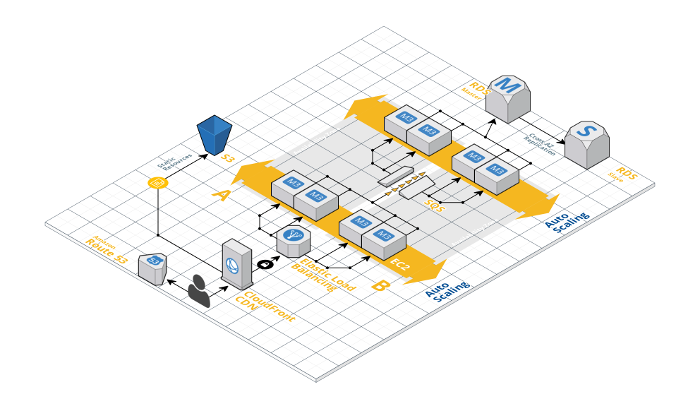
\includegraphics[width=\textwidth]{assets/chapter-2-infrastructure-diagram.png}
	\caption{Contoh gambar}
	\label{fig:contoh_gambar}
\end{figure}

\subsection{Tabel}

Tabel juga merupakan float. Tabel~\ref{table:contoh_tabel} adalah contoh tabel. Perhatikan bahwa walaupun didefinisikan setelah paragraf ini, tabel tidak diletakkan tepat di bawah paragraf ini pada dokumen hasil kompilasi. Hal ini karena ukuran (tinggi) tabel tidak cukup apabila diletakkan di sisa halaman ini. \LaTeX-lah yang mengatur peletakan tabel. Oleh karena itu tidak disarankan untuk merujuk tabel (dan objek float lain) dengan frasa ``Tabel di bawah ini'', ``Tabel berikut'', dan sebagainya.

\begin{table}[htbp]
	\centering
	\caption{Contoh Tabel}
	\label{table:contoh_tabel}
	\begin{tabular}{ll}
		\toprule
		\multicolumn{1}{l}{\textbf{Contoh Judul Kolom}} & \multicolumn{1}{l}{\textbf{Nilai}} \\
		\midrule
		Besaran 1                                       & 12 meter                           \\
		Besaran 2                                       & $360^\circ$                        \\
		Besaran 3                                       & 0,2 meter                          \\
		Besaran 4                                       & $1^\circ$                          \\
		Besaran 5                                       & 8000 sampel/detik                  \\
		\bottomrule
	\end{tabular}
\end{table}

\section{Persamaan Matematika}

Persamaan~\eqref{eq:contoh_equation} adalah contoh persamaan matematika,

\begin{align}
	c^2 = a^2 + b^2\,.
	\label{eq:contoh_equation}
\end{align}

Contoh penggunaan notasi custom,

\begin{align}
	\bayes{x}{y}\,.
	\label{eq:contoh_equation_custom}
\end{align}

\section{Menulis Algoritma dan Pseudocode}

Blok algoritma dan \textit{pseudocode} secara teknis juga merupakan sebuah float. Untuk dapat menggunakan algoritma ada beberapa \textit{package} yang perlu di-\textit{import} (sudah ter-\textit{import} di dokumen ini): \texttt{algorithm} dan \texttt{algpseudocode}. Algoritma \ref{alg:example} adalah contoh blok algoritma.

\begin{algorithm}
	\begin{algorithmic}[1]
		\Function{Example\_algorithm}{$a,b,c$}
		\State $p \gets [~]$
		\For {$a_i \in a$}
		\If{$a_i > 0$}
		\State $p_i \gets a_i + b$
		\Else
		\State $p_i \gets a_i - c$
		\EndIf
		\EndFor
		\State \Return $p$
		\EndFunction
	\end{algorithmic}
	\caption{Contoh Algoritma}
	\label{alg:example}
\end{algorithm}

\section{Studi Terkait}
\blindtext

\documentclass[../index.tex]{subfiles}

\begin{document}

\chapter{SYSTEM DEVELOPMENT METHODOLOGY}

This chapter will define the development methodology which acts as a guideline to fulfil the goals
and objectives of the project. The selected methodology will be justified based on how the
methodology will help the development of the project. It will be followed by the explanation of the
phases of the selected methodology. Then, the system requirements will be analysed in order to be
able to develop a reliable system. The chapter will be ended by the conclusion of the previous
discussion regarding the selected methodology, development phases based on the selected methodology,
and system requirement analysis for the project development.

\section{Methodology Selection and Justification}

The primary objective of this project is to successfully develop a hardware firewall which home
users can use to secure their local network. As this project will only involves infrastructure
design, system integration, and configuration of existing software and technology without any
application development, the waterfall model is selected as the development methodology. Waterfall
model is selected as the proposed system will mainly serve its function with minimal user-facing
interface. This is in accordance with the definition of waterfall model where the product definition
is required to be stable among the course of the development. Another reason is the project involves
hardware development or configuration where manufacturing or procurement cost are involved. In
addition, the developed system appliance could be considered as critical system which requires
extensive safety and security analysis of the solution specification and design \cite{Balaji_2012}.

\section{Phases of Selected Methodology}

The Waterfall model is a linear and sequential software development process consisting of several
phases. The Waterfall model initiated with Requirement Gathering and Analysis, followed by System
Design, Implementation, Integration and System Testing, and ended with Deployment and Maintenance.

\subsection{Requirements Gathering and Analysis}

The Waterfall project methodology is started by gathering the project requirements and analyse the
collected facts. The system services, constraints, and objectives are established with the system
users. They are then defined in detail and serve as a system specification.

For this project, this phase will discuss several network security concerns that exist in home
network environment. After the issues and concerns have been identified, the possible solution or
countermeasures will be discussed. The outcome of the discussion for this phase should be used as
the reference for considerations and justifications in later phases.

This project has gathered the potential issues that exist in home network environment in Chapter 1
and further discussed it in Chapter 2. Followed by that, the possible solution and improvement of
the gathered issues and concerns has been explored. The outcome of the discussion for this phase
will be used as the reference for considerations and justifications in following system development
phases.

\subsection{System Design}

Following the Requirements Gathering and Analysis is the System Design phase. This phase defines the
required condition to either software or physical hardware systems.  This involves identifying the
modules or components of the system, their relationships, and how they will interact with each
other. It determines the entire system architecture in general view.

The System Design phase will be discussed in Chapter 4 of the project report. In this phase, the
proposed system design will be defined based on the result of the Requirement Gathering and Analysis
phase. Both of the hardware and software implementation which will include system infrastructure
design and programs and subsystems that are going to be utilised will be discussed and proposed to
be applied in following system development phases.

\subsection{Implementation}

The Implementation phase is where the design is finalised as a set of solution or components. This
also includes verification that every implemented components fulfill its requirements.

In this phase, any infrastructure and software design  based on the outcome of Requirement Analysis
and System Design phases will be developed and configured. Initially, the proposed system
infrastructure will be built in accordance to the proposed System Design. After the proposed system
infrastructure has been established, the software can start to be installed and configured based on
the gathered requirements.

\subsection{Integration and System Testing}

In the Integration and System Testing phase, the particular solution or components are configured
and assembled as one entire system. To guarantee that the project requirements have been fulfilled,
the project may only proceed to the Deployment and Maintenance phase after the proposed system has
been thoroughly tested for its functionality.

In Integration and System Testing phase, the developed system will be tested based on the defined
testing methodology. This phase will ensure that both the hardware and software aspect of the system
is running properly and provide security to the home network according to the system design.

\subsection{Deployment and Maintenance}

After the previous phases of system development, design, implementation, and testing have been done
and passed, the proposed system will be deployed to be used based on its use cases and requirements.
After the proposed system has been successfully deployed, the project will move to the Maintenance
phase. This phase will involve addressing user feedback, fixing defects or issues discovered after
deployment, and making necessary updates or enhancements.

The Deployment phase of this project will involve the integration of the proposed system in an
existing home network environment such as IP addressing and network bridging based on the deployment
environment. Afterwards, the deployed system will be observed for any issues found during the usage
which will be addressed in the Maintenance phase.

\section{Technology Used}

To achieve the project objectives defined in previous chapter, the following technology will be
used:

\subsection{Proxmox VE}

Proxmox VE is a type 1 hypervisor which serves as server management platform for enterprise
virtualization. It operates directly on a bare-metal system by utilizing the Linux Containers (LXC)
and KVM hypervisor as well as software-defined networking and storage. All of that features are
implemented on a single platform.

Proxmox will be used as the base foundation of the proposed system. It allows other subsystems such
as OPNsense virtual machine and containers for Pi-hole and the monitoring stack to be installed in
one PC.

\subsection{OPNsense}

OPNsense is an open-source firewall and routing platform based on FreeBSD. A few of its features
including traffic shaping, forward caching proxy, OpenVPN client and intrusion detection system.

OPNsense will be used as primary firewall OS of the proposed system. It will provide the network-
based firewall and network routing for the local network. A necessary configuration is required to
fulfill the project objectives which will be further discussed in Chapter 5.

% \subsection{LXC}
%
% LXC is one of type 1 hypervisor technology used to run multiple separate Linux system in the form of
% container on a control host which utilize single Linux kernel.
%
% LXC is selected to be used for the project as it has minimal overhead compared to other deployment
% method. Instead of creating an entire virtual machine, LXC achieves its virtualization by utilizing
% virtual environment which has separate network and process space.
%
% In the system development project, LXC will be use for the deployment of Pi- hole application.
% Instead of virtualizing the entire operating system only for Pi-hole, LXC can be utilized to provide
% the necessary virtualization with noticably lower overhead.

\subsection{Pi-hole}

Pi-hole is a DNS server that has DNS sinkhole feature which protects devices connected to the local
network from unwanted content, such as advertisement and internet tracker, without being required to
install any client-side software.

In this project, Pi-hole will be implemented in the proposed system as an advertisement and internet
tracker blocker. Any DNS query will be sent to Pi-hole and Pi-hole will determine if the DNS queries
should be forwarded or allowed or it should be blocked based on the applied rules.

% \subsection{Telegraf}

\subsection{Vector}

Vector is a data processing pipeline that allows logs and metrics collection, transformation, and
routing. One of the advantage of Vector compared to its alternatives is that it has wide
compatibility with various data source and output sink vendor which make it easier to integrate and
utilise in different environments.

Vector will be used in the proposed system to filter and sanitise syslogs that will be received from
other VM and containers. Afterwards, the processed logs will be shipped to Loki for log storage.

\subsection{Loki}

Grafana Loki is a log aggregation and storage system which took inspiration from Prometheus. Loki
allows for efficient indexing of log data as in Loki index is copmrised from labels without the
original log message.

Loki will be used to store the syslog data which is forwarded by OPNsense and Pi-hole that consists
of firewall action, Suricata IDS, and DNS block log. This log will be used as the data source for
Grafana dashboard.

\subsection{Prometheus}

Prometheus is a system monitoring and alerting toolkit which retrieves and stores metrics along with
the timestamp at when it was reported and optional labels.

\begin{figure}[h]
  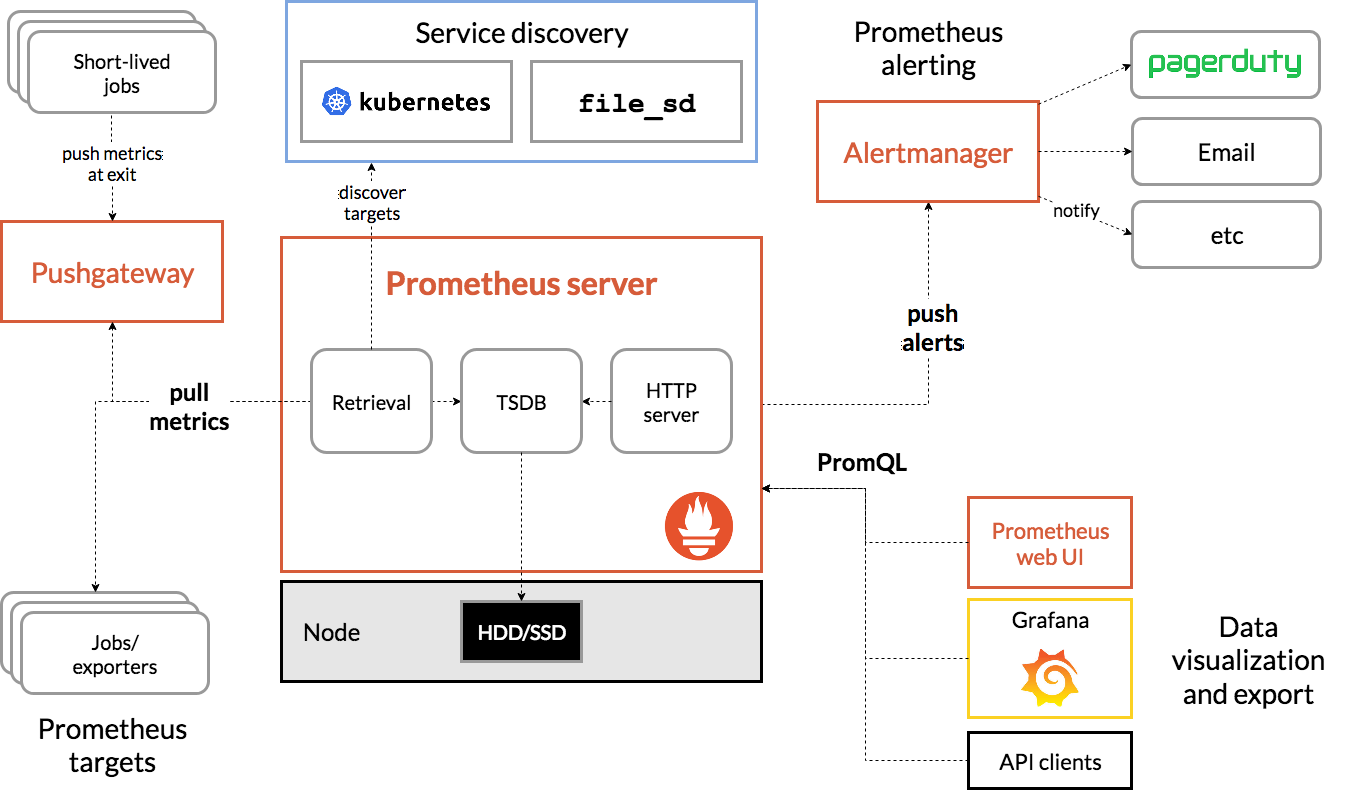
\includegraphics[width=\textwidth]{../assets/prometheus_architecture.png}
  \caption{Prometheus architecture}
  \label{fig:prometheus_architecture}
\end{figure}

\Cref{fig:prometheus_architecture} shows the architecture of Prometheus. Prometheus works by
scraping metrics from instrumented jobs, either directly or through an intermediary push gateway for
ephemeral jobs. It locally stores all scraped metrics and applies rules throughout this data to
enable log aggregation and recording of new time series from existing data or alerts generation.
Afterwards, this time series can be used by Grafana or other API consumers to visualize the
collected data.

Prometheus will be used to scrape and store the metrics of OPNsense VM and Pi-hole container. This
metric will be used by Grafana to create centralised monitoring dashboard.

\subsection{Grafana}

Grafana is an open-source data visualization and monitoring tool used to create interactive and
customizable dashboards for analyzing and monitoring various data sources. It allows users to query,
visualize, and understand data from different systems and applications through a unified and
intuitive interface.

In this project, Grafana will be used to create centralised monitoring dashboard. This includes
VM and container system metrics, network access log, firewall action log, and DNS block log. This
centralised monitoring dashboard allows system administrator monitors the proposed system simpler
and easier.

\section{System Requirement}

This section refers to the process of identifying and specifying the hardware, software, and network
requirements for a particular system or software application. It involves understanding the
necessary resources and capabilities that a system needs to operate effectively and efficiently.

To ensure that the proposed system met the project objectives and able to deliver its functionality
as optimal as possible, several requirements have been determined.

\subsection{Hardware Requirement}

% The main objective of this project is to develop a low-cost hardware firewall by utilizing an old
% PC. As PC is becoming more accessible to every person, it is chosen as the base hardware which the
% firewall and additional application will be deployed.

\begin{table}[H]
  \begin{tblr}{width=\textwidth,colspec={|X[c,m]|X[l,m]|X[l,m]|}}
    \hline
    \SetCell[c=1]{c} Hardware & \SetCell[c=1]{c} Specification & \SetCell[c=1]{c} Justification \\
    \hline
    Laptop & {OS: Windows 11 64-bit \\ CPU: AMD Ryzen 7 4800H 8c16t \\ RAM: 32GB DDR4 \\ Storage:
    2TB NVME SSD} & Environment for project research, development, and maintenance with the
    specified hardware is required to for smooth development \\ 
    \hline
    Proposed System Host & {OS: Proxmox VE 64-bit \\ CPU: Intel Core i5 8600T 6c6t \\ RAM: 16GB DDR4
    \\ Storage: 512GB NVME SSD, 512GB SATA HDD} & Environment for project research, development, and
    maintenance with the specified hardware is required to for smooth development \\ 
    \hline
  \end{tblr}
  \caption{Hardware requirements}
  \label{table:hardware_requirements}
\end{table}

\Cref{table:hardware_requirements} shows the hardware requirements for both laptop to help with
development phase and proposed system host.

\subsection{Software Requirement}

\begin{table}[H]
  \begin{tblr}{width=\textwidth,colspec={|X[c,m]|X[l,m]|}}
    \hline
    \SetCell[c=1]{c} Software & \SetCell[c=1]{c} Justification \\
    \hline
    Neovim & IDE and Documentation writing \\
    Ventoy & Creation of bootable USB \\
    Ansible & Configuration management / Infrastructure as Code \\
    TeX Live & Documentation writing \\
    Google Chrome & Access web GUI of proposed system \\
    Windows Subsystems for Linux & Subsystem to run Linux on Windows \\
    \hline
  \end{tblr}
  \caption{Software requirements}
  \label{table:software_requirements}
\end{table}

\Cref{table:hardware_requirements} shows the hardware requirements for both laptop to help with
development phase and proposed system host.

\section{Summary}

This chapter discussed the detailed steps for the implementation or developments of the proposed
system. Technologies and system requirement which covers both hardware and software requirements are
defined further. Clearly defining the methodology and system requirements will help to ensure the
project is completed and its objectives and deliverable are achieved within the allocated period.
The system requirement, both software and hardware, also discussed for the purpose of keeping the
system running optimally. This chapter discussed the detailed steps for the implementation or
developments of the proposed system. Technologies and system requirement which covers both hardware
and software requirements are defined further. Clearly defining the methodology and system
requirements will help to ensure the project is completed and its objectives and deliverable are
achieved within the allocated period. The system requirement, both software and hardware, also
discussed for the purpose of keeping the system running optimally.

\end{document}

\documentclass[../index.tex]{subfiles}

\begin{document}

\chapter{REQUIREMENT ANALYSIS AND DESIGN}

This chapter will examine the proposed project requirements and system design. Identifying project
requirements and defining the proposed system design are mandatory to successfully deliver the
project objectives and functionalities.

\section{Requirement Analysis}

Unified Modeling Language (UML) is chosen as a method to analyze the project requirements. UML is a
graphically based notation, which is developed by the Object Management Group as a standard means of
describing software-oriented designs. It contains several different types of diagrams, which allow
different aspects and properties of a system design to be implemented.

% However, for this particular project, only a few of UML diagrams will be used. This due to the
% project development does not involve any creation of new software or interface. Rather, this
% project implements off-shelf software solutions in a defined hardware.

The functional requirements are described using UML use case diagram and activity diagram. The
non-functional requirement will review the performance, usability, availability, reliability, and
security aspect of the system.

\subsection{Functional Requirement}

This section will outline the specific features, capabilities, and behavior that the software system
should possess in order to fulfill its intended purpose and meet the needs of its users. The
functional requirements describe what the system should do, rather than how it should be
implemented.

\subsubsection{Use Case Diagram}

Use case diagram is a visual depiction of a user's possible interactions with a certain system. A
use case diagram defines varying use cases and different types of users the system has and commonly
delivered with other types of diagrams as well. Use case diagram offers thorough summary of the
entire system with simple illustration. Use case diagram is also considered as the perfect method to
provide the overall view of the system at the early stage \cite{Shen2003FormalizationTA}.

\begin{figure}[h]
  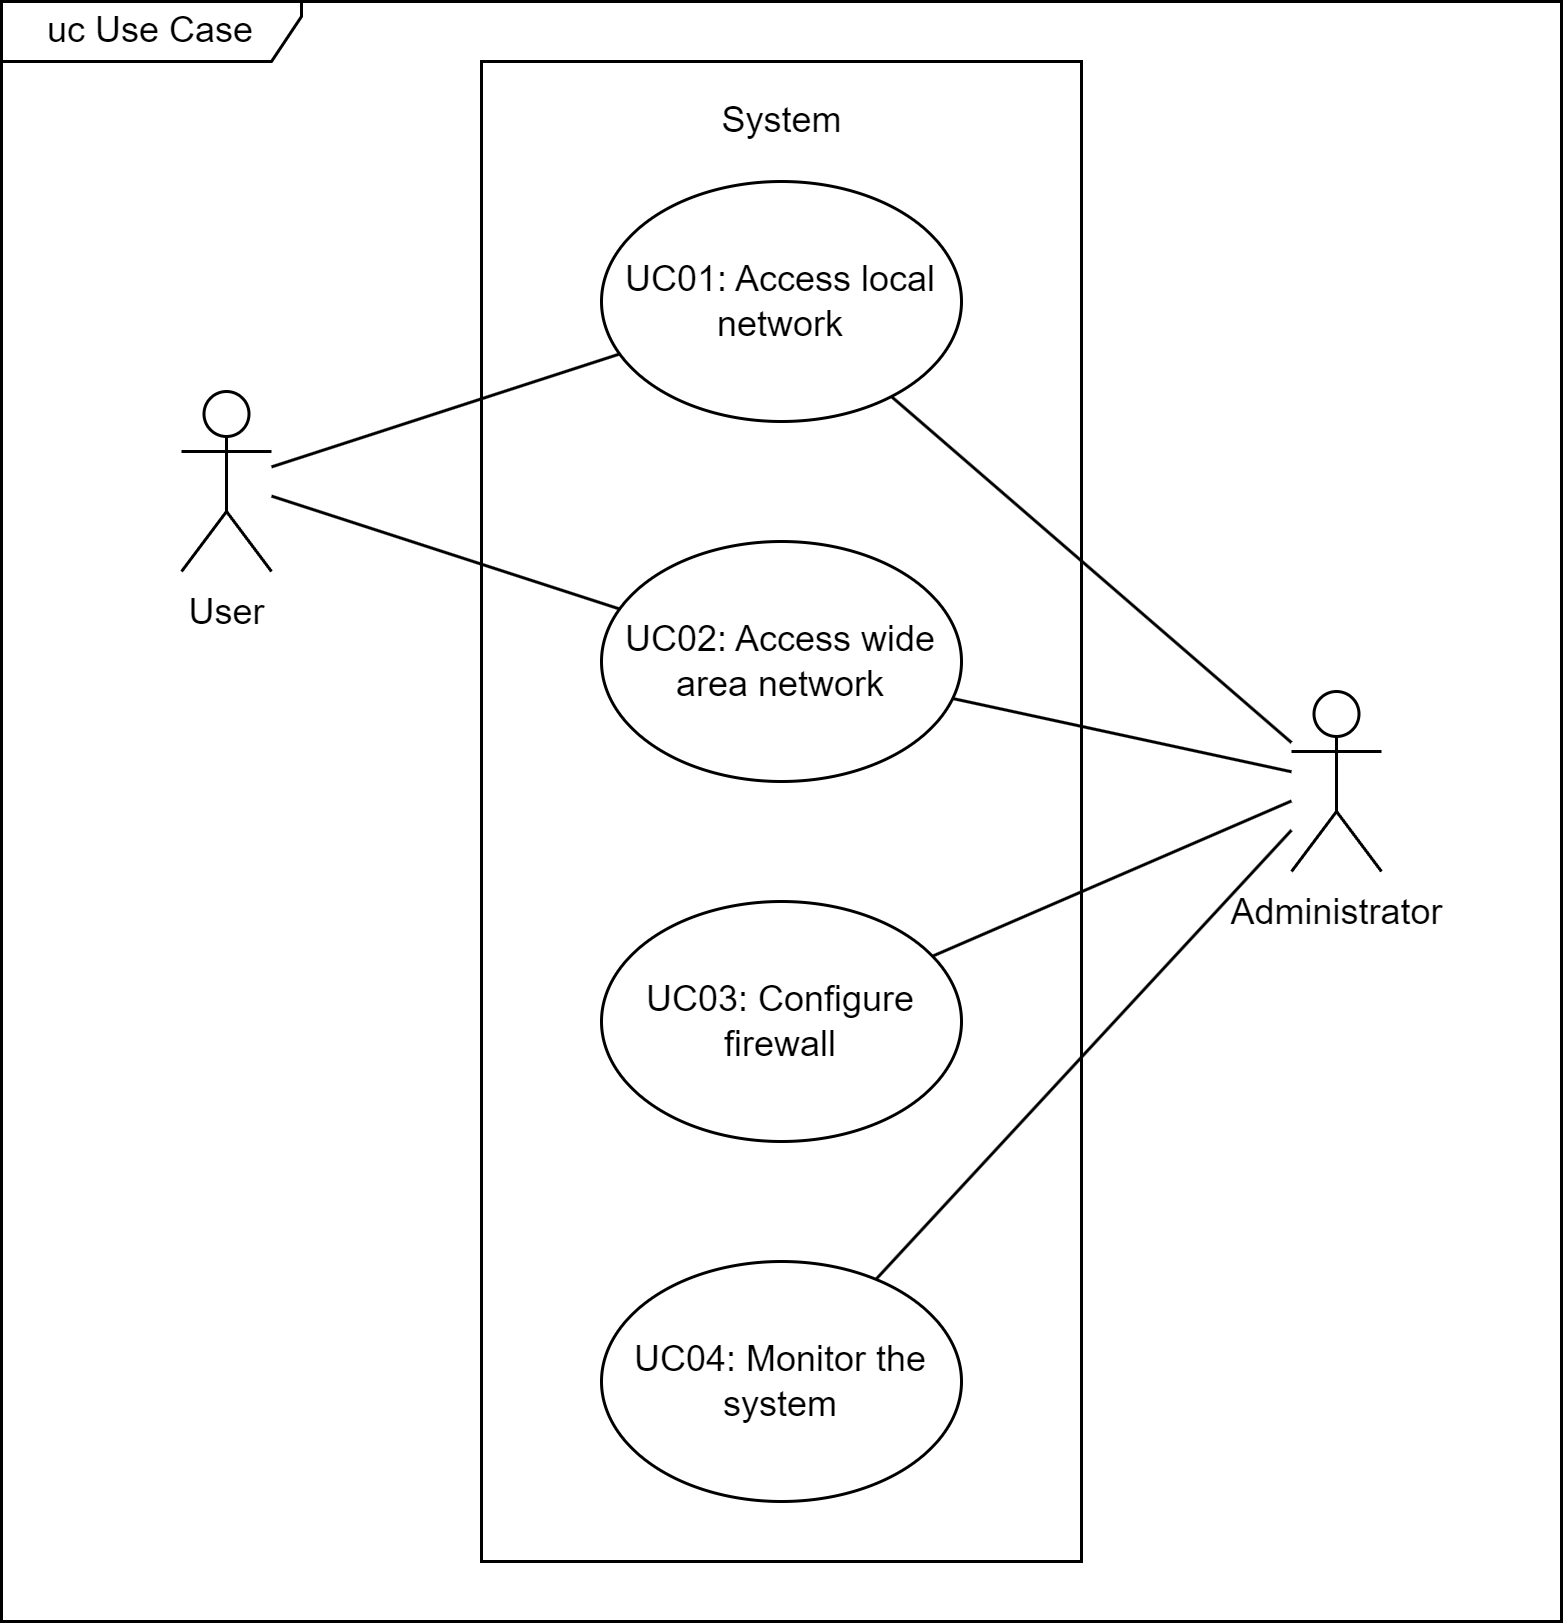
\includegraphics[width=\textwidth]{../assets/use_case.drawio_2.png}
  \caption{Use case diagram of the proposed system}
  \label{fig:use_case}
\end{figure}

\Cref{fig:use_case} shows the use case diagram of the proposed system. The use case diagram is
designed based on the result of the requirement analysis phase. In the proposed system, there exist
three actors which are the user, the system, and the administrator. Four use cases were also
defined, which are accessing local area network, accessing wide area network, configuring the firewall,
and monitoring the system. In addition, it followed by a table which list the brief use case
description.

\begin{table}[H]
  \begin{tblr}{hlines,width=\textwidth,colspec={|X[l,m]|X[l,m]|}}
    \SetCell[c=1]{c} Use Case & \SetCell[c=1]{c} Description \\
    UC01: Access local area network & User access another device which exists in the local area
    network \\

    UC02: Access wide area network / Internet & User access the Internet \\

    UC03: Configure System & Administrator configure the system using the proposed Ansible playbook
    \\

    UC04: Monitor system & Administrator monitor the system metrics and logs \\
  \end{tblr}
  \caption{Brief description of use case diagram}
  \label{table:use_case}
\end{table}

\Cref{table:use_case} lists all of the use cases identified for the proposed system. The use case
description provides the flow of each use case, alternative flow, the precondition that should be
fulfilled as well as post conditions based on the outcome of the flow. The purpose of defining the
use case description is to present the overall view of the system function and reaction to the user
and administrator. In the proposed system, there are 4 use cases in total which detailed more in
Appendix A.

\begin{table}[H]
  \begin{tblr}{hlines,measure=vbox,width=\textwidth,colspec={|l|X[l,m]|}}
    Use case & Access local network \\
    ID & UC01 \\
    Description & User access another device which exists in the local network \\
    Actor & User, System \\
    Related use case & - \\
    Precondition & User's device is connected to the System \\
    Normal flow &
    \begin{enumerate}
      \item The use case starts whenever User is trying to communicate or access a device in the
        local network

      \item The System receives the request packet from User's device

      \item The System forwards the packet to the appropriate destination, in this case it is the
        device which the User wants to access

      \item The destination address receives the packet

      \item The destination address sends the response packet to the System

      \item The system forwards the packet to appropriate destination, in this case it is the User's
        device
    \end{enumerate} \\
    Alternative flow & - \\
    Post condition &
    \begin{enumerate}
      \item Success condition
        \begin{enumerate}
          \item The User receives the response from the device
        \end{enumerate}
        \item Failure condition
          \begin{enumerate}
            \item The User fails to receive the response from the device

            \item The System drops the packet
          \end{enumerate}
    \end{enumerate} \\
  \end{tblr}
  \caption{Use case description of Access Local Network}
  \label{table:use_case_1}
\end{table}

\subsubsection{Activity Diagram}

As stated by \cite{10.1109/APSEC.2004.55}, activity diagram could be used to model the dynamic
aspects of a group of objects, making it a perfect method to describe the fulfillment of the
operation in the design phase. Activity diagram also suitable to describe the sequence of the
activities among the existing objects in the control flow during the implementation of an operation.
In addition, activity diagram could be used to describe the relationship between the activity and
the object in the system flow as well as the change of state of object in the object flow as the
activity being executed. The following figure shows the activity flow of access local network. The
complete activity diagram of the system is enclosed in Appendix A.

\begin{figure}[h]
  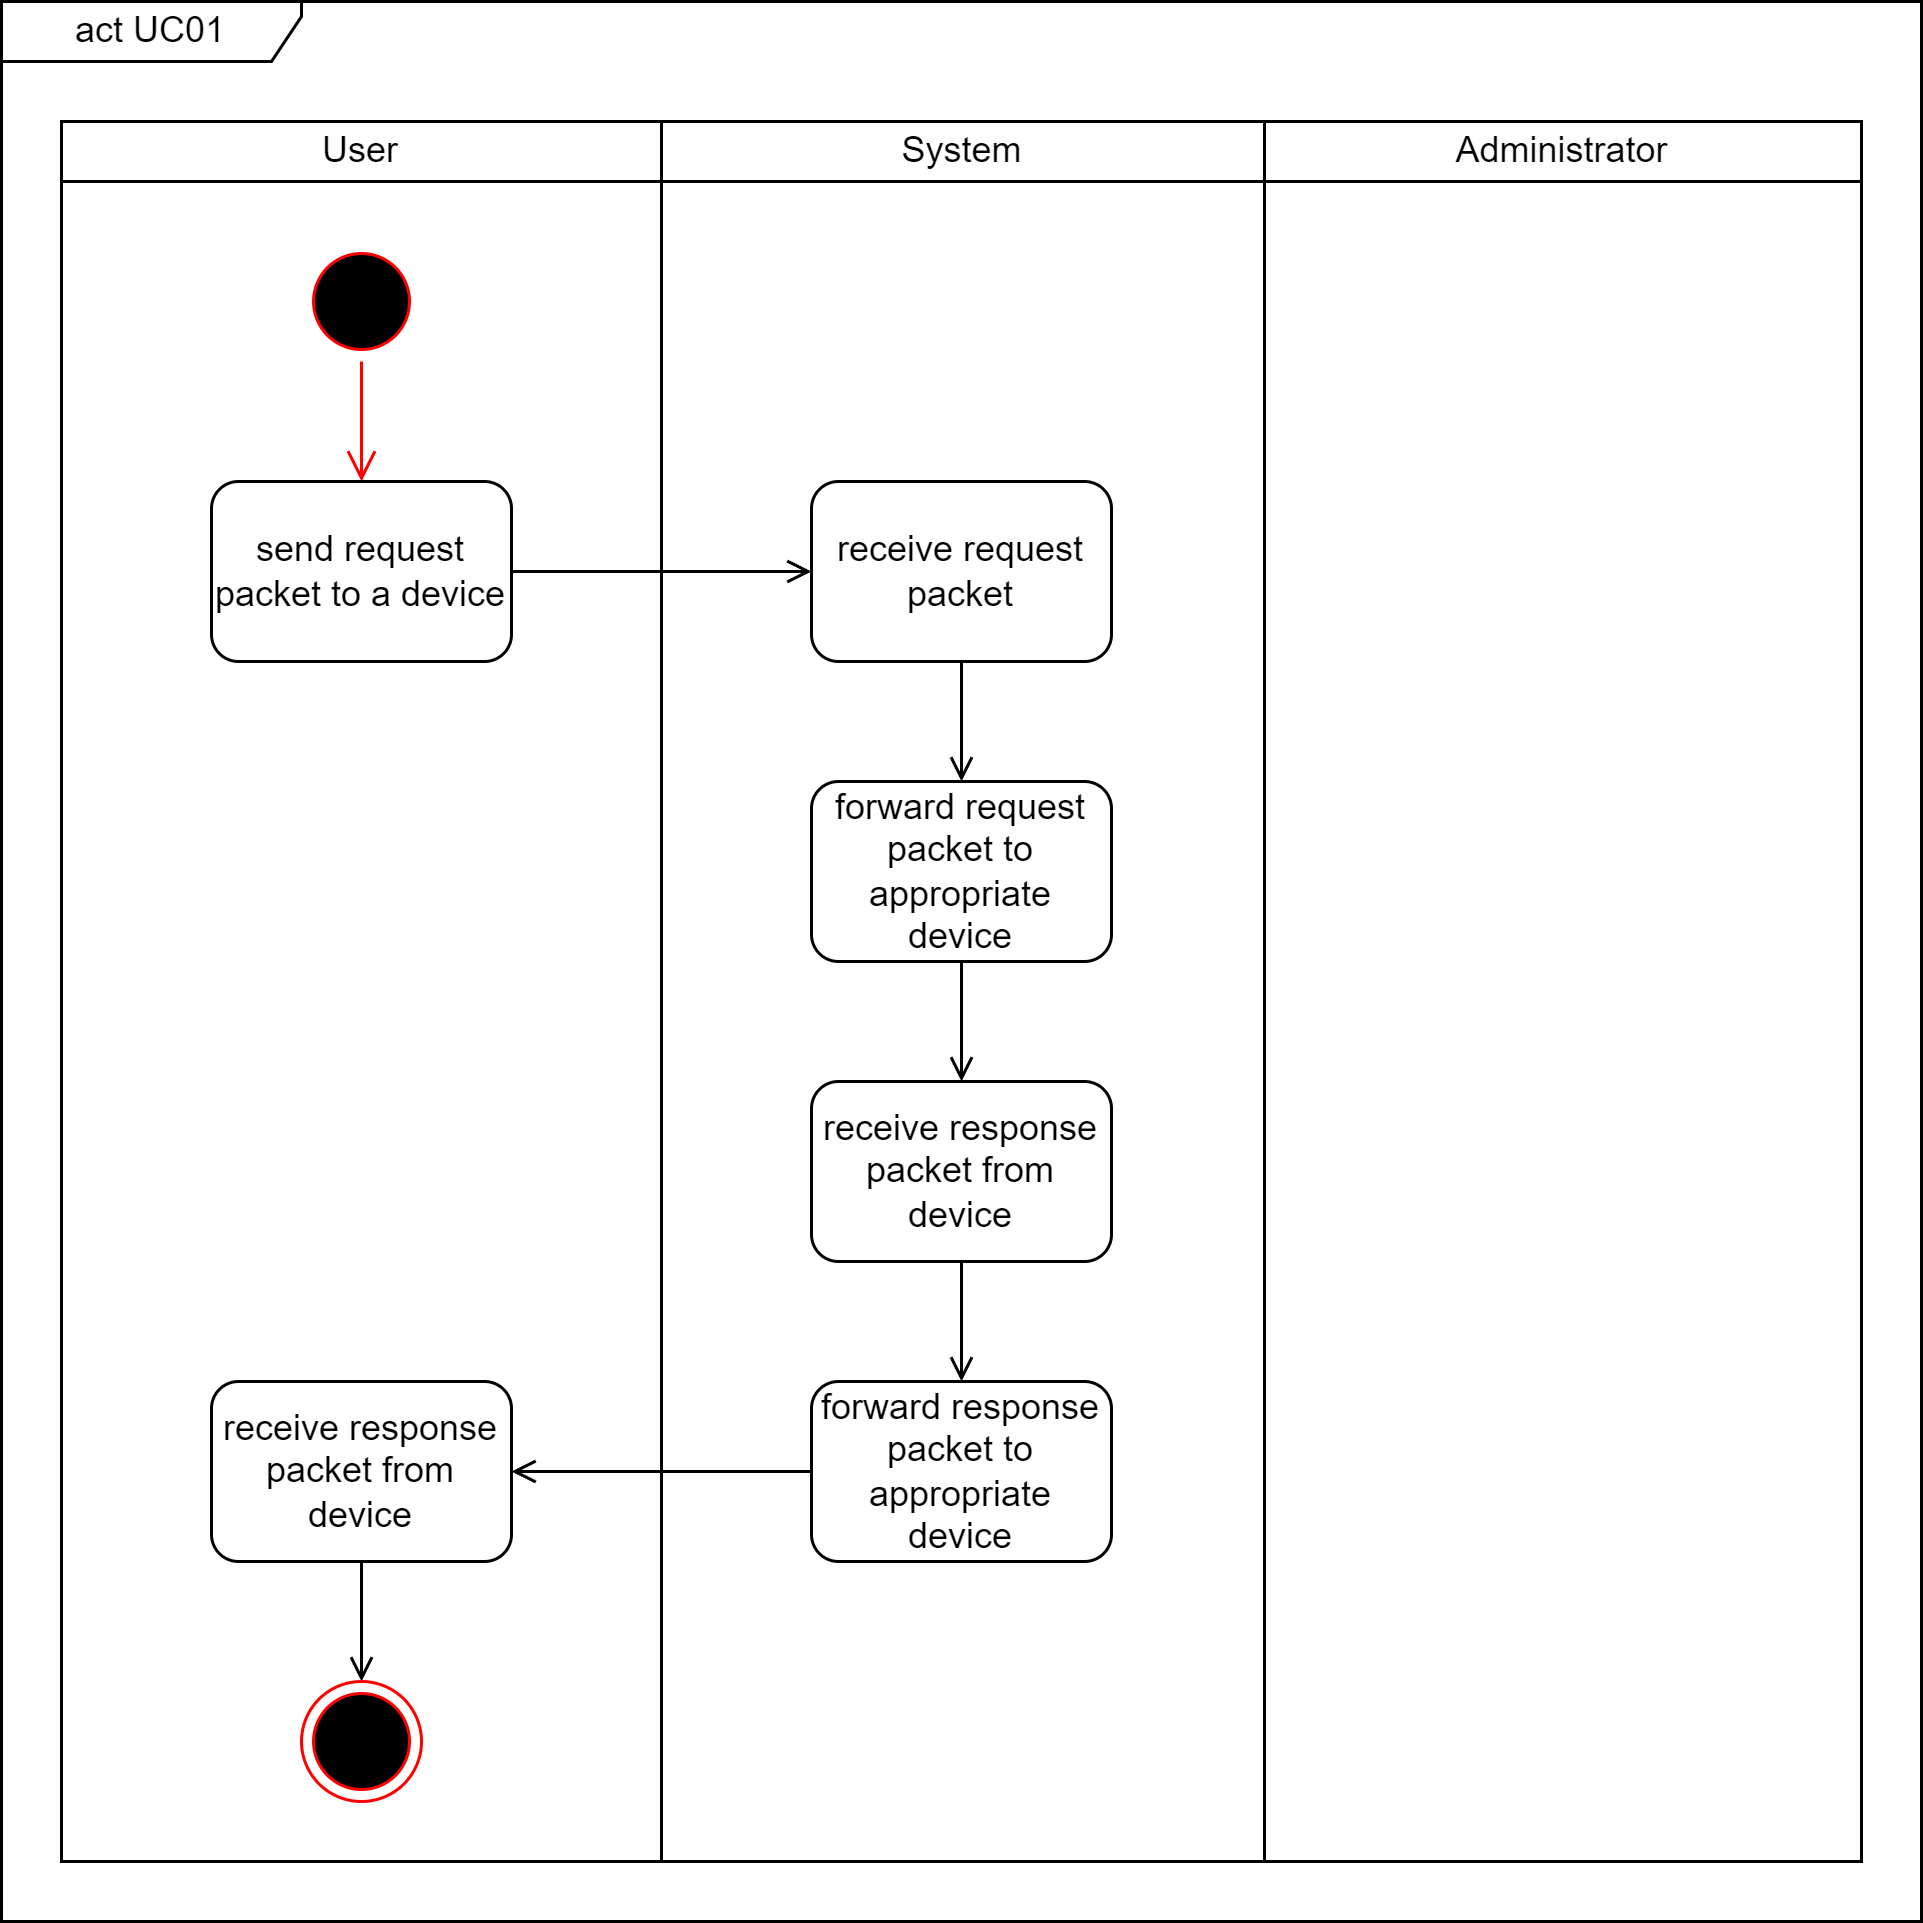
\includegraphics[width=\textwidth]{../assets/activity_diagram.drawio.png}
  \caption{Activity diagram of Access Local Network}
  \label{fig:activity_diagram_1}
\end{figure}

\subsection{Non-functional Requirement}

The non-functional requirement describes the measurement of quality of the system, consisting of
system performance, usability, availability, reliability, and security

For the system performance, the developed system should be able to transmit over 900 Mbps. This is
due to the NIC used, which is limited to 1 Gbps. As for the system usability, the administrator
should be able to modify the configuration of the firewall based on their requirement. As the system
will act as both internet router and network firewall without high availability (HA), the system is
expected to be able to run 24 hours a day, seven days a week. The error budget is only allocated for
the system maintenance. Aside securing the local network, the system also required to have certain
kind of self-security functionality to be able to defend itself from attacks

% \section{Project Design}
\section{Infrastructure Design}

The system will utilize Proxmox VE which act as server management platform as its base. Proxmox VE
provides KVM hypervisor, storage and network virtualization for the system. The Proxmox VE will
manage virtualised OPNsense host and local Kubernetes cluster in parallel. The OPNsense host will
provide the main network firewall and routing capabilities. The Pi-hole will be deployed on an LXC
container.

\begin{figure}[h]
  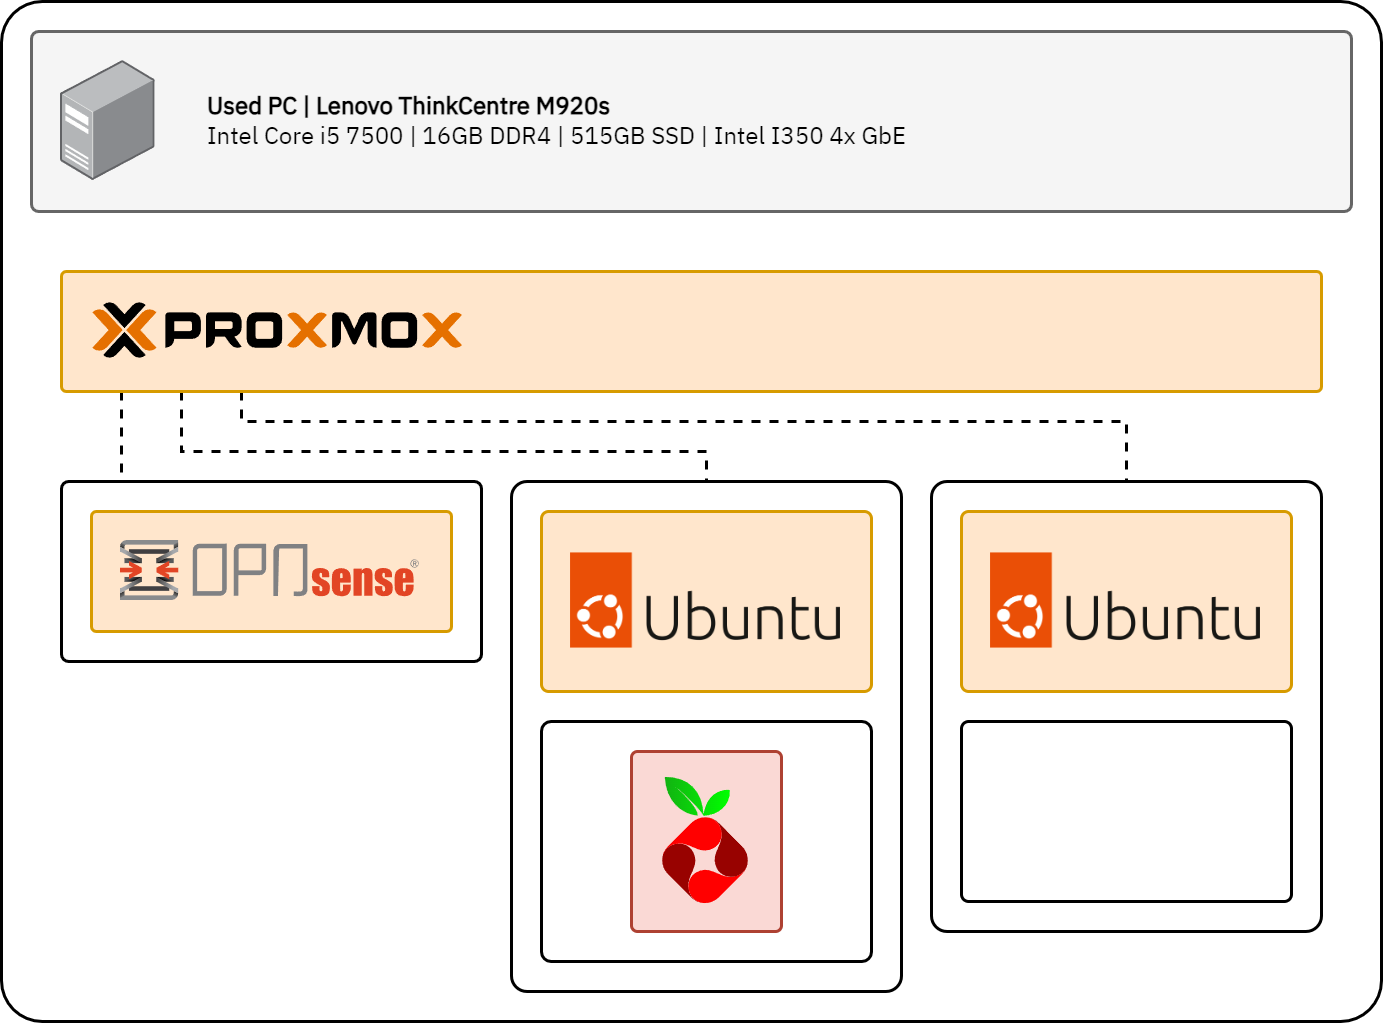
\includegraphics[width=\textwidth]{../assets/project_design.drawio.png}
  \caption{Proposed system infrastructure design}
  \label{fig:project_design}
\end{figure}

\section{Network Design}



\section{Summary}

This project uses different approach for its requirement analysis and system design. This chapter
does not include proposed software design as the proposed system development does not involve the
creation of a new software or application, rather designing and re-purposing or configuring a
hardware to make it usable as alternative for firewall appliances which have significantly higher
price tag.

\end{document}

\chapter{PENUTUP}

\section{Kesimpulan}
\blindtext

\section{Saran}
\blindtext

%----------------------------------------------------------------%

% Daftar pustaka
\begingroup
\renewcommand{\baselinestretch}{1.0}
\printbibliography[heading=bibintoc]
\endgroup

% Before:
% ---
% Index
% \appendix
% \addcontentsline{toc}{part}{Lampiran}
% \part*{Lampiran}
% ---

% Format judul bab lampiran
\titleformat{\chapter}[hang]
{\large\bfseries}
{\chaptertitlename\ \thechapter}{1em}
{\large\bfseries}
\titlespacing*{\chapter}{0pt}{-1.5\baselineskip}{\parskip}

\begin{appendices}
	\documentclass[../index.tex]{subfiles}

\begin{document}

\chapter{Instrumen Pengujian}

\end{document}

	\chapter{Rincian Kasus Uji}

\end{appendices}

\end{document}
